% Initial config
\documentclass[12pt,a4paper]{report}
\usepackage[utf8]{inputenc}
\usepackage{glossaries-extra}

% Title and authors
\title{End of Studies Project}
\author{
    Anis, Benna\\
    \texttt{anis.benna@incedo.com}
    \and
    Firas, Jaber\\
    \texttt{firas.jaber@incedo.com}
}
\date{March 2022}

% Import packages
\usepackage{pdfpages}
\usepackage{natbib}
\usepackage{graphicx}
\usepackage{float}
\usepackage{tabularx}
\usepackage{colortbl}
\usepackage{multirow}
\usepackage{caption}
\usepackage{chngcntr}
\usepackage[hyphens]{url}
\usepackage{listings}
\usepackage{color}
\usepackage{textcomp}
\usepackage[toc,page]{appendix}
\usepackage{ragged2e}
\usepackage{enumitem}
\usepackage[parfill]{parskip} % \medskip and \noindent are not needed. See https://tex.stackexchange.com/a/74173/268270
\usepackage{fancyhdr}
\usepackage{minitoc}

% DEVONLY:
% \usepackage{lipsum} % Lorem ipsum

% Glossary list
% \newglossaryentry{latex}
% {
%     name=latex,
%     description={Is a mark up language specially suited
%             for scientific documents}
% }
% \newglossaryentry{maths}
% {
%     name=mathematics,
%     description={Mathematics is what mathematicians do}
% }

% List of acronyms
\newacronym{ilg}{ILG}{Incedo Lead Generator}
\newacronym{saas}{SaaS}{Software as a Service}
\newacronym{poc}{POC}{Proof of Concept}
\newacronym{vm}{VM}{Virtual Machine}
\newacronym{iac}{IaC}{Infrastructure as Code}

% NOTE: Using acronyms in the document
% \glsxtrlong{ilg} => Incedo Lead Generator
% \glsxtrshort{ilg} => ILG
% \glsxtrfull{ilg} => Incedo Lead Generator (ILG)

% \acrlong{ilg} \acrshort{ilg} \acrfull{ilg} can also be used but should not in our current setup.
% See https://tex.stackexchange.com/questions/318694/glossaries-acronyms-avoid-additional-entries-in-number-list-with-indexonlyfirs


% ------------- Document content ------------- %
\begin{document}

% Global config
% Color palette
\definecolor{primary}{cmyk}{0, 0.23, 0.98, 0.17}
\definecolor{secondary}{cmyk}{0.48, 0.16, 0, 0.61}

% Global Figure and Table count
\counterwithout{figure}{chapter}
\counterwithout{table}{chapter}


% Include the cover page
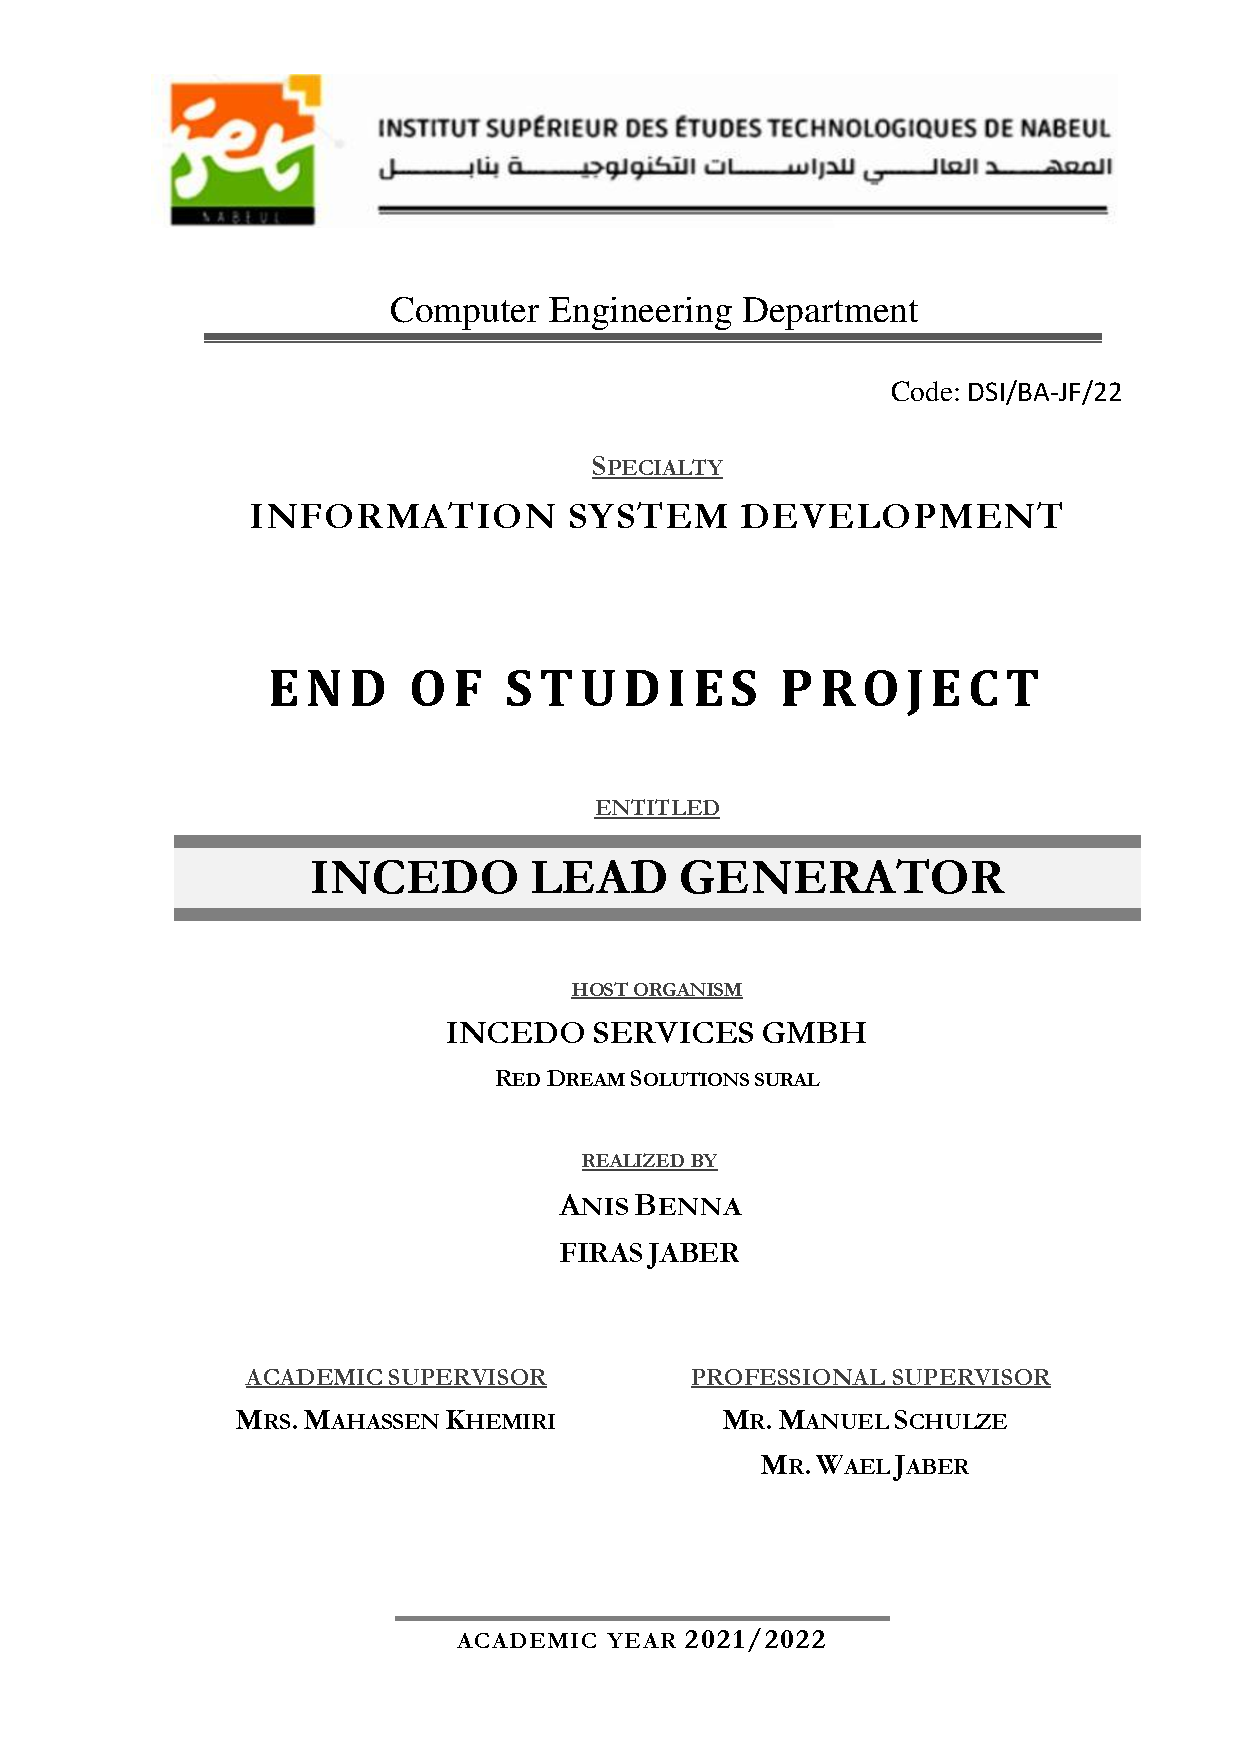
\includepdf[]{src/assets/pdfs/cover-page.pdf}

% Set page numbering to roman for initial pages
\pagenumbering{roman}
\setcounter{page}{1}

% Dedication and acknowledgments
% \section*{Dedication}
\lipsum[1-3]
\newpage

\section*{Dedication}
\lipsum[1-3]
\newpage
 % Optional
\section*{Acknowledgments}
We would like to take a moment to thank all of those involved in finalizing this work, whether directly or indirectly.

% Thanking the Incedo team
Our profound gratitude goes to the entire \textbf{Incedo Services GmbH team} for their warm welcome, invaluable support and for accompanying us throughout this wonderful journey.
Special thanks to our company supervisor and product owner \textbf{Mr. Manuel Schulze} who has been very involved with us almost daily throughout the long period of the internship, his trust in us has truly allowed us to come very far during this project.
We also appreciate \textbf{Wael Jaber} for initially showing us the ropes and for his continuous guidance.
Our deepest gratefulness also goes to \textbf{Mr. Robert Könitz} and \textbf{Mr. Tobias Schulze} for their huge efforts in contributing to our weekly mentoring sessions amongst other things, their input has truly been a huge source of knowledge for both of us and will be forevermore.
We would also like to thank both of \textbf{Mrs. Mai Ly Moll} and \textbf{Mrs. Xenia Harter} for their efforts in business development and for organizing the delightful team events that we gladly had the occasion to participate in, as well as for their almost daily engagements that don't fall short from our supervisor's. We also extend our thanks to the rest of the Incedo team \textbf{Mr. Joachim Liedtke}, \textbf{Mr. Mohamed Elloumi} and \textbf{Mr. Gabor Kluge}.

% Thanking the University supervisor
We also wish to acknowledge the great support of our university supervisor \textbf{Mrs. Mahassen Khemiri} for her assistance, availability and valuable spot-on advice.
Her faith in us has truly allowed us to keep working on this project stress-free while confident this report will turn out better than initially intended.

Our heartfelt appreciation goes to the jury members who agreed to evaluate our work and we hope they find it up to standard.
We equally thank all of the teachers of the Higher Institute of Technological Studies of Nabeul (ISETN) who contributed to our education during these wonderful two and a half years.

% \medskip
% \noindent We would also like to take this opportunity to express how joyful we are to keep working as official permanent team members of Incedo!

\newpage


% Abstract or TL;DR
\section*{Abstract}
The Incedo Lead Generator or ILG for short is a proprietary software solution of Incedo Services GmbH that's offered in a software as a service modal or SaaS.
It scrapes LinkedIn and uses it as a medium to directly automate the generating of leads from a campaign using the LinkedIn sales navigator feature.

\medskip
\noindent To start off, we have two big roles to play.
\textbf{The first} one is to develop new features for the existing software solution while continuously monitoring the changes LinkedIn makes (since we rely on scraping).
\textbf{The second} and the most important one is to migrate ILG from a monolithic application to a \textbf{microservices} architecture in order to make it infinitely scalable. We also have to find the ideal environment to deploy our newly created microservices to, in order to ensure their intra-communication.

\medskip
\noindent We start by breaking our application into various NestJS microservices, build the corresponding docker images then create a shared Helm package for the microservices. Second of all, we setup our own \textbf{self-managed Kubernetes cluster with MicroK8s and ansible scripts}, configure it appropriately to support our specific use-case, then deploy our application stack to both staging and production.

\medskip
\noindent Lastly, using \textbf{GitLab's CI/CD pipelines} and also \textbf{GNU's Makefiles} allows us to automate the whole process from start to finish. So that in the end, one commit on the main branch is enough to deliver our changes to the clients, which is the standard that \textbf{DevOps compliant} applications should follow.

\newpage


% Print the acronyms list
\printunsrtglossaries
\newpage

% Tables
\renewcommand{\contentsname}{Table of Contents}
\tableofcontents
\listoffigures \mtcaddchapter % https://tex.stackexchange.com/questions/155177/how-to-add-the-word-figure-to-the-list-of-figures
\listoftables \mtcaddchapter % https://tex.stackexchange.com/questions/79869/first-chapter-after-list-of-tables-starts-on-page-2-should-be-1
\clearpage

% Set page numbering to Arabic for main content
\pagenumbering{arabic}

% Include the main app
% Main Document
\maketitle
%\section{Introduction}
There is a theory which states that if ever anyone discovers exactly what the Universe is for and why it is here, it will instantly disappear and be replaced by something even more bizarre and inexplicable \cite{databaseII}.
There is another model which states that this has already happened.

\section{Methodology}
This is the methodology section.

\section{Results}
This is the results section.

\begin{figure}[h!]
    \centering
    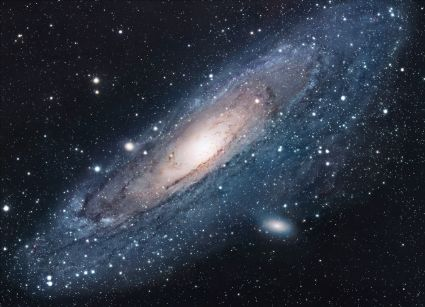
\includegraphics[scale=1.7]{src/assets/images/universe}
    \caption{The Universe}
    \label{fig:universe}
\end{figure}

\section{Conclusion}
``I always thought something was fundamentally wrong with the universe'' \citep{adams1995hitchhiker}

\chapter{ General framework}
\setcounter{secnumdepth}{3}
\newpage

\section*{Introduction}
\addcontentsline{toc}{section}{Introduction}
This chapter introduces the general context of this report. We start by presenting the frame of the project as well as the host company. Then comes the enumeration of the problems which led to the realization of the project. We wrap it up by defining the methodology we’ve followed to carry out our work. \citep{test1}

\section{General framework of the internship}
\addcontentsline{toc}{section}{General framework of the internship}
This project was carried out within the frame of obtaining a bachelor’s degree in Computer Science at the Higher Institute of Technological studies of Nabeul. The internship took place fully remotely at Incedo Services GmbH for five months starting from the 1st of February 2022 to the 30th of June 2022 with the purpose of further developing the existing project as well as slowly migrating it to a micro-services architecture. \cite{test2}

\section{Company overview}
\addcontentsline{toc}{section}{Company overview}
This section introduces the host company and its offered services.
\subsection{About Incedo}
\subsection{Incedo Services}

\section{Stating the problem}
\addcontentsline{toc}{section}{Company overview}
Incedo -having ambitious goals to grow over the next 2 to 4 years- wants to win new clients and strategically develop the existing ones. Winning new clients starts with generating new leads. Previously, Incedo has worked with an Austrian start-up (motion group) that provides automated lead generation through LinkedIn at the cost of 0.85 € per requested contact in LinkedIn. Although one big project was closed and several leads were generated, Incedo started using the LinkedIn Sales Navigator with a more targeted approach, but nevertheless wanted to automate the approach and increase its outreach.
Having launched the first version of the ILG (Incedo Lead Generator) as a SaaS (Software as Service), Incedo was satisfied for a while. Over the time however, as more and more clients were interested in the ILG, the current architecture couldn’t handle the load properly.

\section{Assessment of the case}
\addcontentsline{toc}{section}{Assessment of the case}
\subsection{Describing the work procedure}
The work on any project must first of all be preceded by a thorough study of the existing ones which undermines the strengths and weaknesses of the current system, as well as the business decisions that should be taken into account during the conception as well as the realization.
\subsection{Criticizing the current state}
After studying the existing, we can determine its limitations:
\begin{itemize}
	\item Bugs always tend to happen whenever the LinkedIn website changes (due to scraping).
	\item Since cron jobs are running for the whole day, bugs are hard to respond to fast enough because we can only deploy once at the end of day.
	\item It is hard to test the whole workflow because of how the app works (looking for certain changes in the LinkedIn interface after certain buttons are clicked for example) meaning that the dev environment is lacking.
	\item It cannot scale well enough since the whole application is deployed on a single server.
\end{itemize}
\subsection{Proposed solution}
% NOTE: Fix New Paragraph identation
The solution to these problems is refactoring the whole application to separate sub applications (microservices) where the automation and scraping processes can be scaled independently of the other parts of the application.

\medskip
This way, it will be easier to maintain and scale the different codebases as well as respond faster to bugs and know exactly what caused them in the first place.


\newpage
\section{Assessment of the case}
\addcontentsline{toc}{section}{Assessment of the case}
\subsection{Agile methodology}
Agile is a structured and iterative approach to project management and product development. It recognizes the volatility of product development, and provides a methodology for self-organizing teams to respond to change without going off the rails.
\subsection{Scrum methodology}
Scrum teams commit to completing an increment of work, which is potentially shippable, through set intervals called sprints. Their goal is to create learning loops to quickly gather and integrate customer feedback. Scrum teams adopt specific roles, create special artifacts, and hold regular ceremonies to keep things moving forward.
\subsection{Kanban methodology}
Kanban is all about visualizing your work, limiting work in progress, and maximizing efficiency (or flow). Kanban teams focus on reducing the time a project takes (or user story) from start to finish. They do this by using a kanban board and continuously improving their flow of work.
\subsection{The choice for ILG}
Kanban is based on a continuous workflow structure that keeps teams nimble and ready to adapt to changing priorities. Work items—represented by cards— are organized on a kanban board where they flow from one stage of the workflow(column) to the next. Common workflow stages are To Do, In Progress, In Review, Blocked, and Done. And since this project is very susceptible to changes from outside (LinkedIn), Kanban offered more flexibility than Scrum so that’s why the team went with it instead.




% Generate a webography, for more styles
% see - https://www.overleaf.com/learn/latex/Bibtex_bibliography_styles#Table_of_stylename_values
\renewcommand\bibname{Webography}
\bibliographystyle{plain}
\bibliography{references}
\addcontentsline{toc}{chapter}{Webography}
\clearpage

% % Set page numbering to alphabetic for appendices
\pagenumbering{alph}
\setcounter{page}{0}

% Very big diagrams, pictures or schemas go here
% List of appendices
\begin{appendices}
    % Appendix a
    \section{ILG Campaign management}
    \begin{figure}[H]
        \centering
        \makebox[\textwidth]{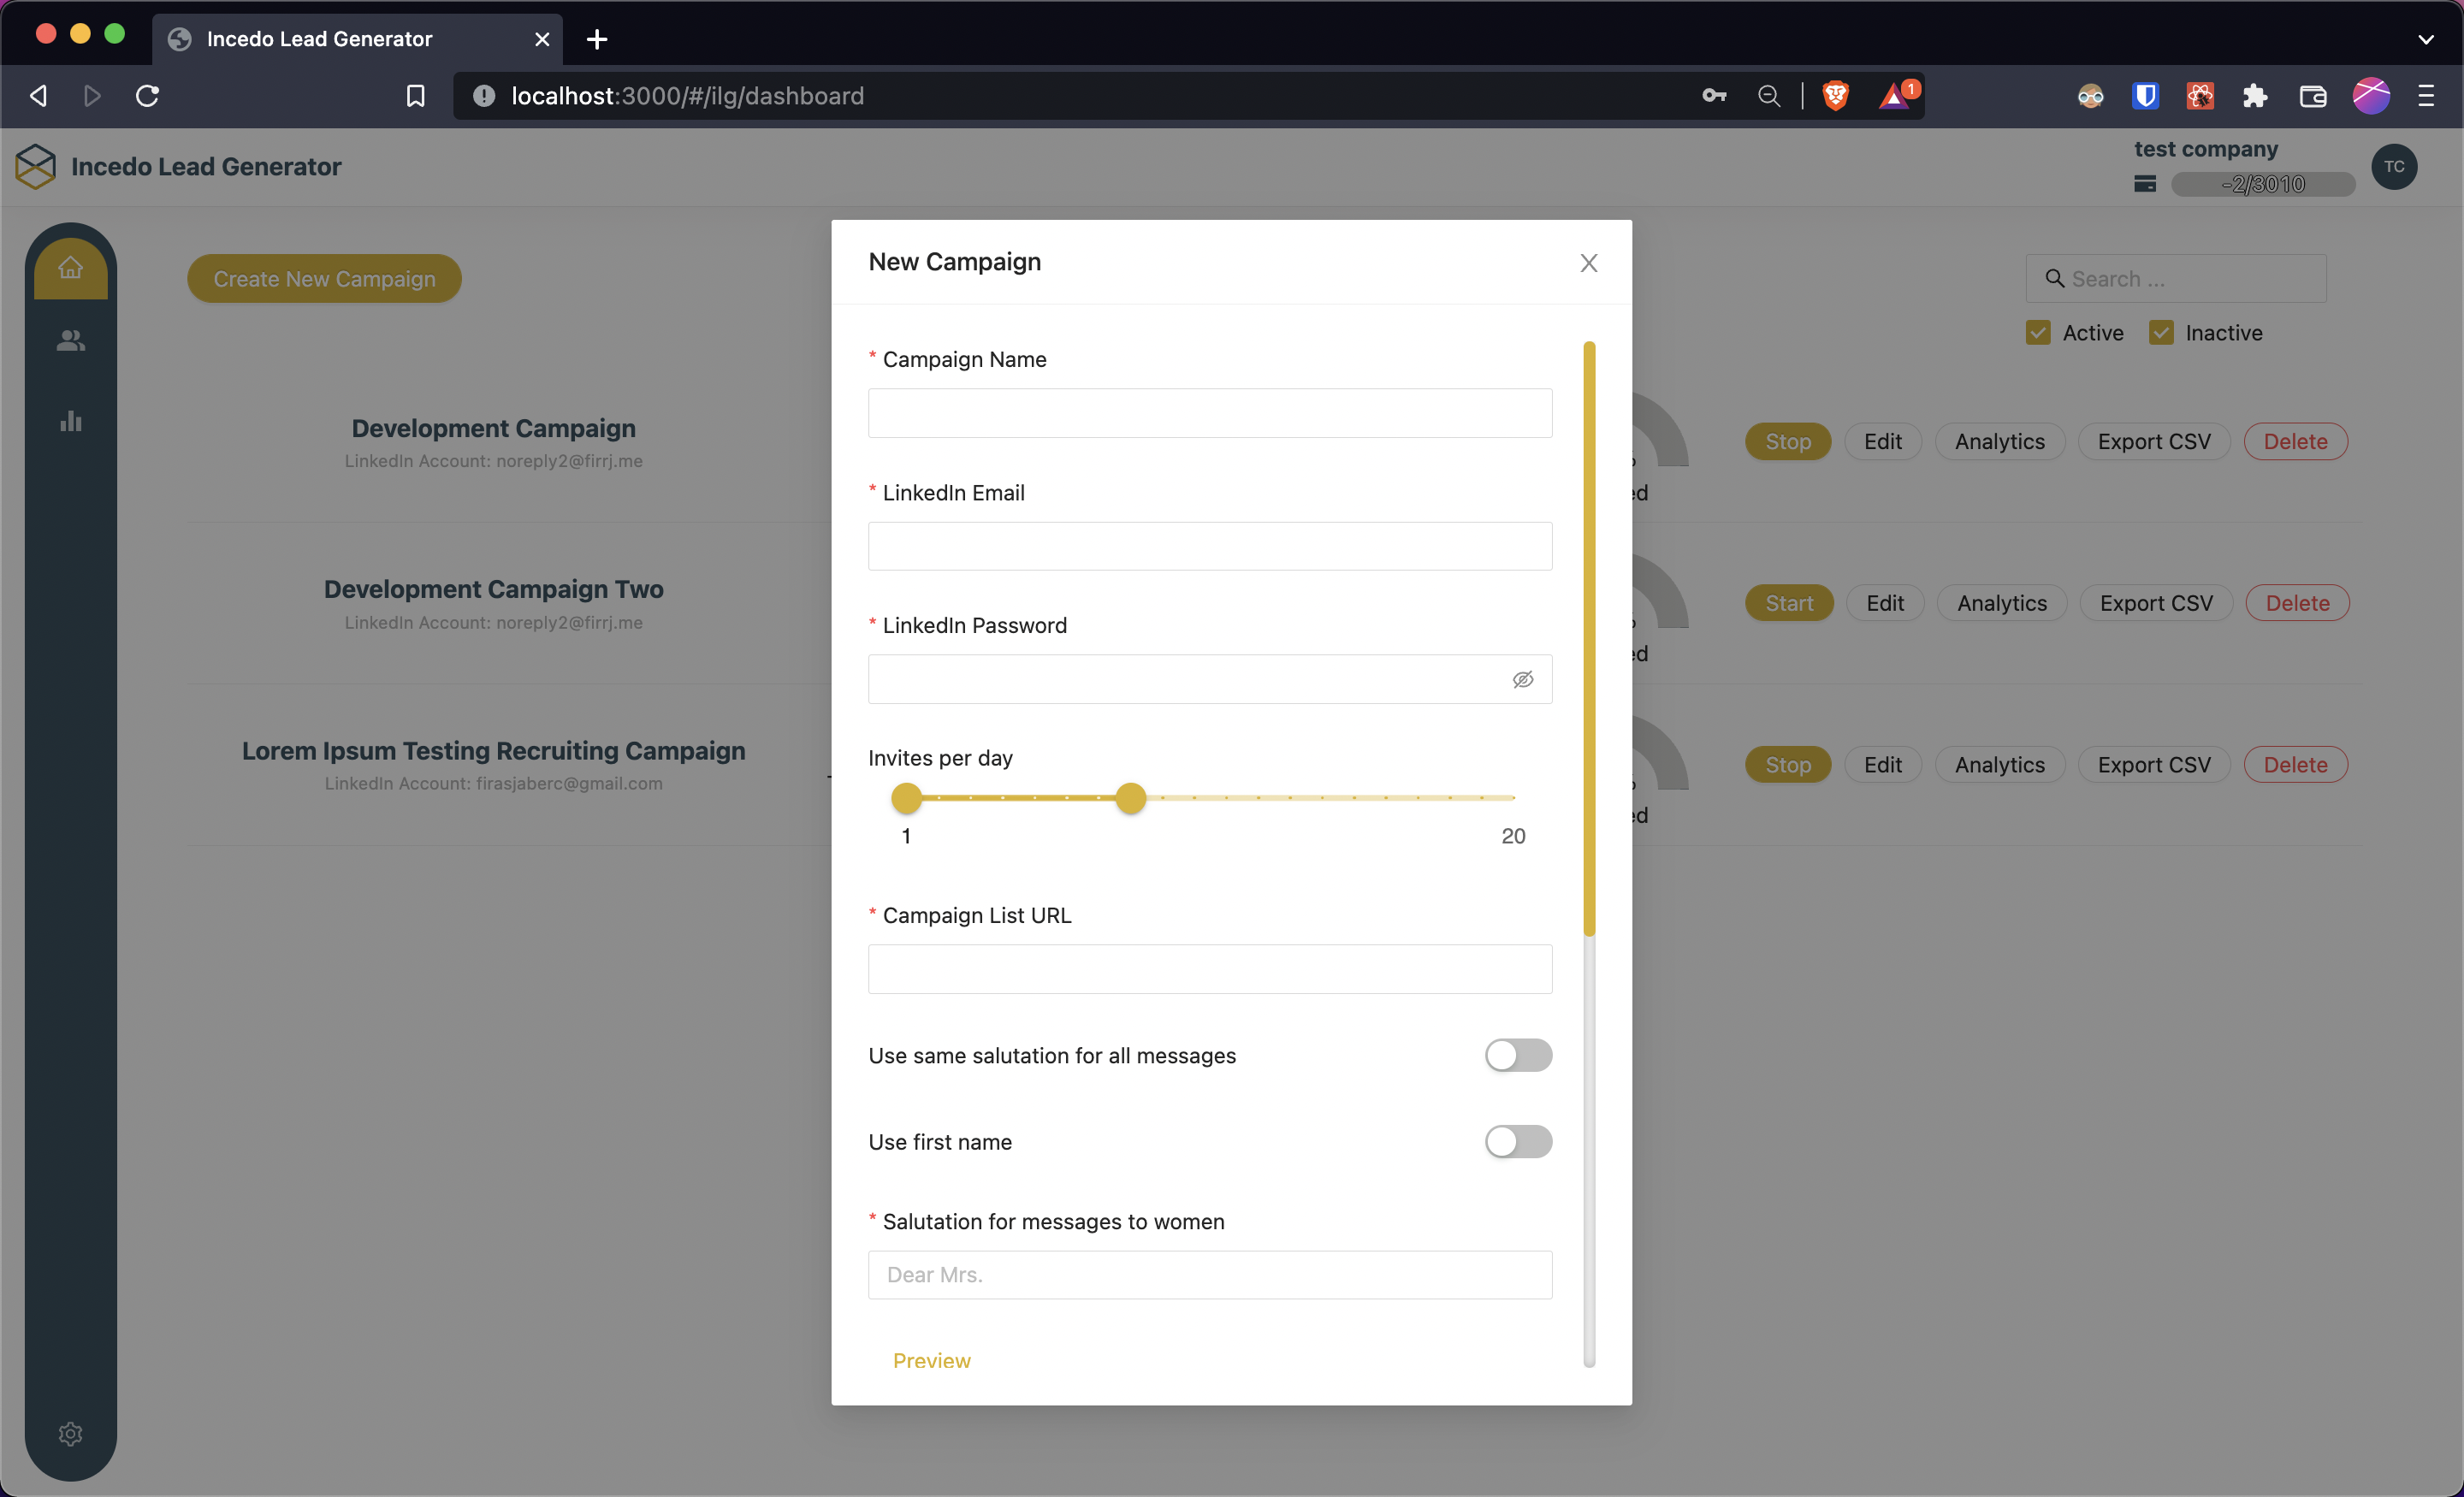
\includegraphics[width=\linewidth]{src/assets/app-screenshots/campaigns-add.png}}
        \caption*{Add campaign form}
    \end{figure}
    \begin{figure}[H]
        \centering
        \makebox[\textwidth]{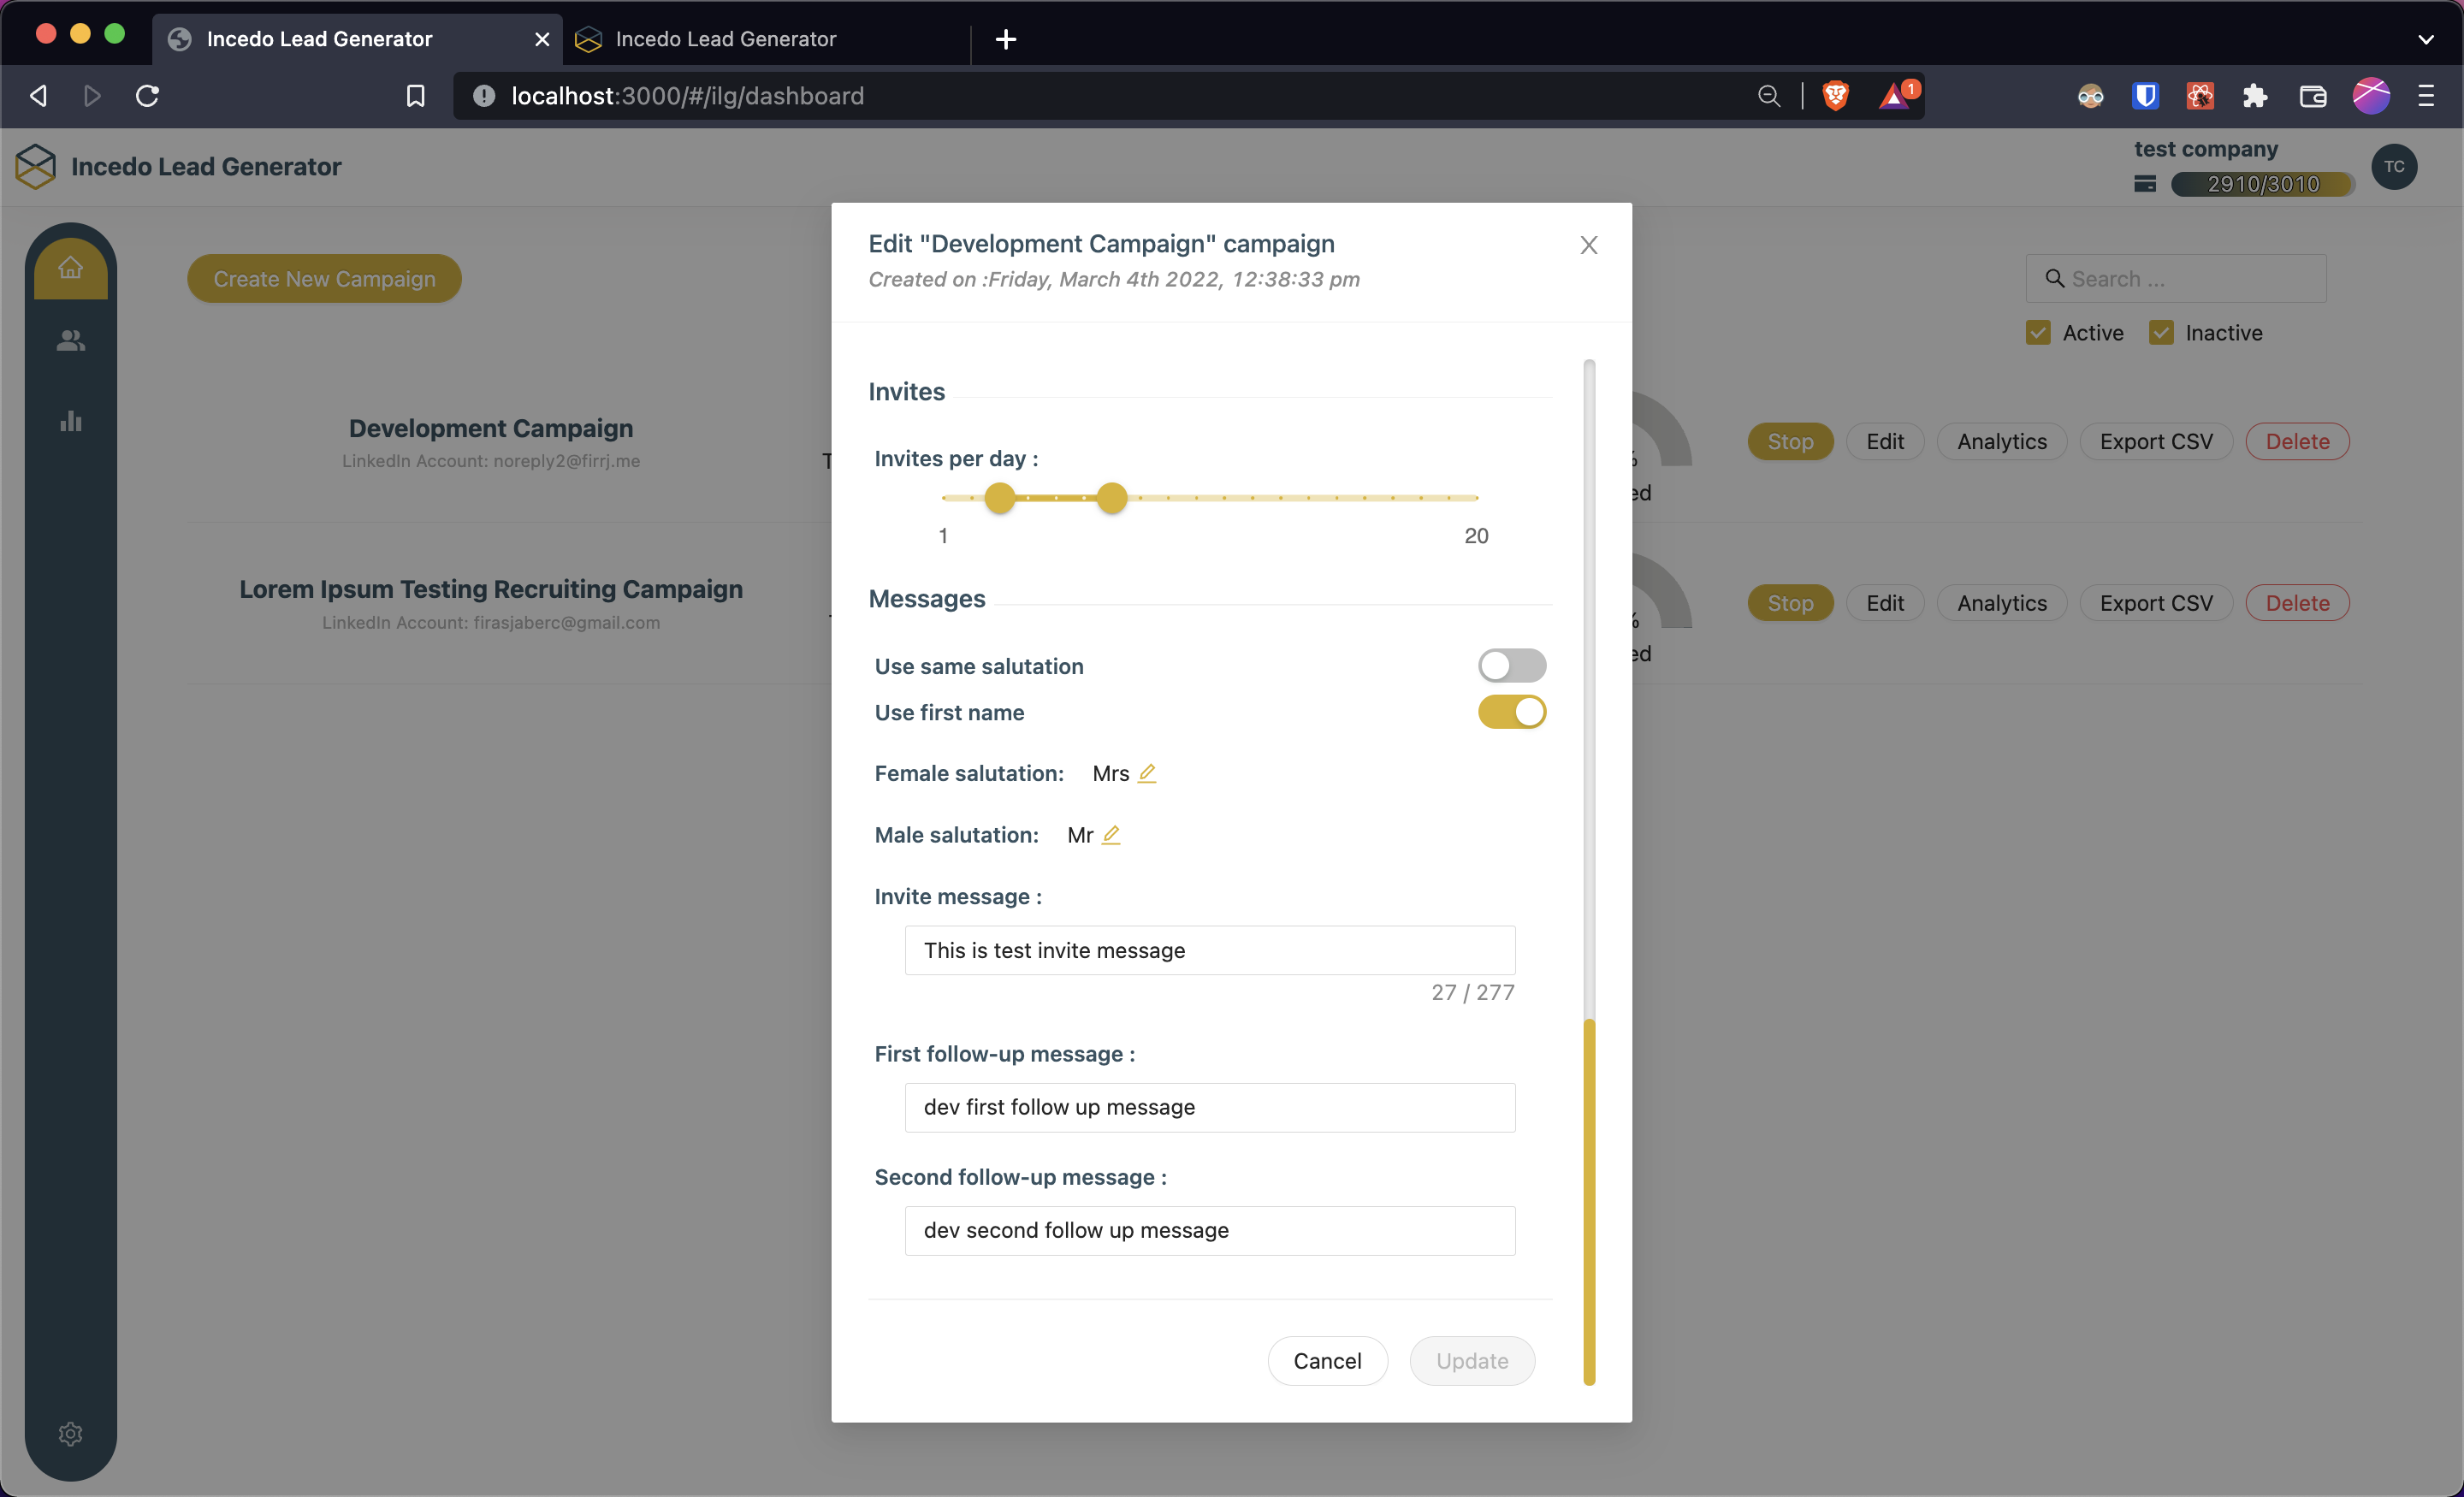
\includegraphics[width=\linewidth]{src/assets/app-screenshots/campaigns-edit.png}}
        \caption*{Edit campaign form}
    \end{figure}

    % Appendix b
    \section{ILG User management}
    \begin{figure}[H]
        \centering
        \makebox[\textwidth]{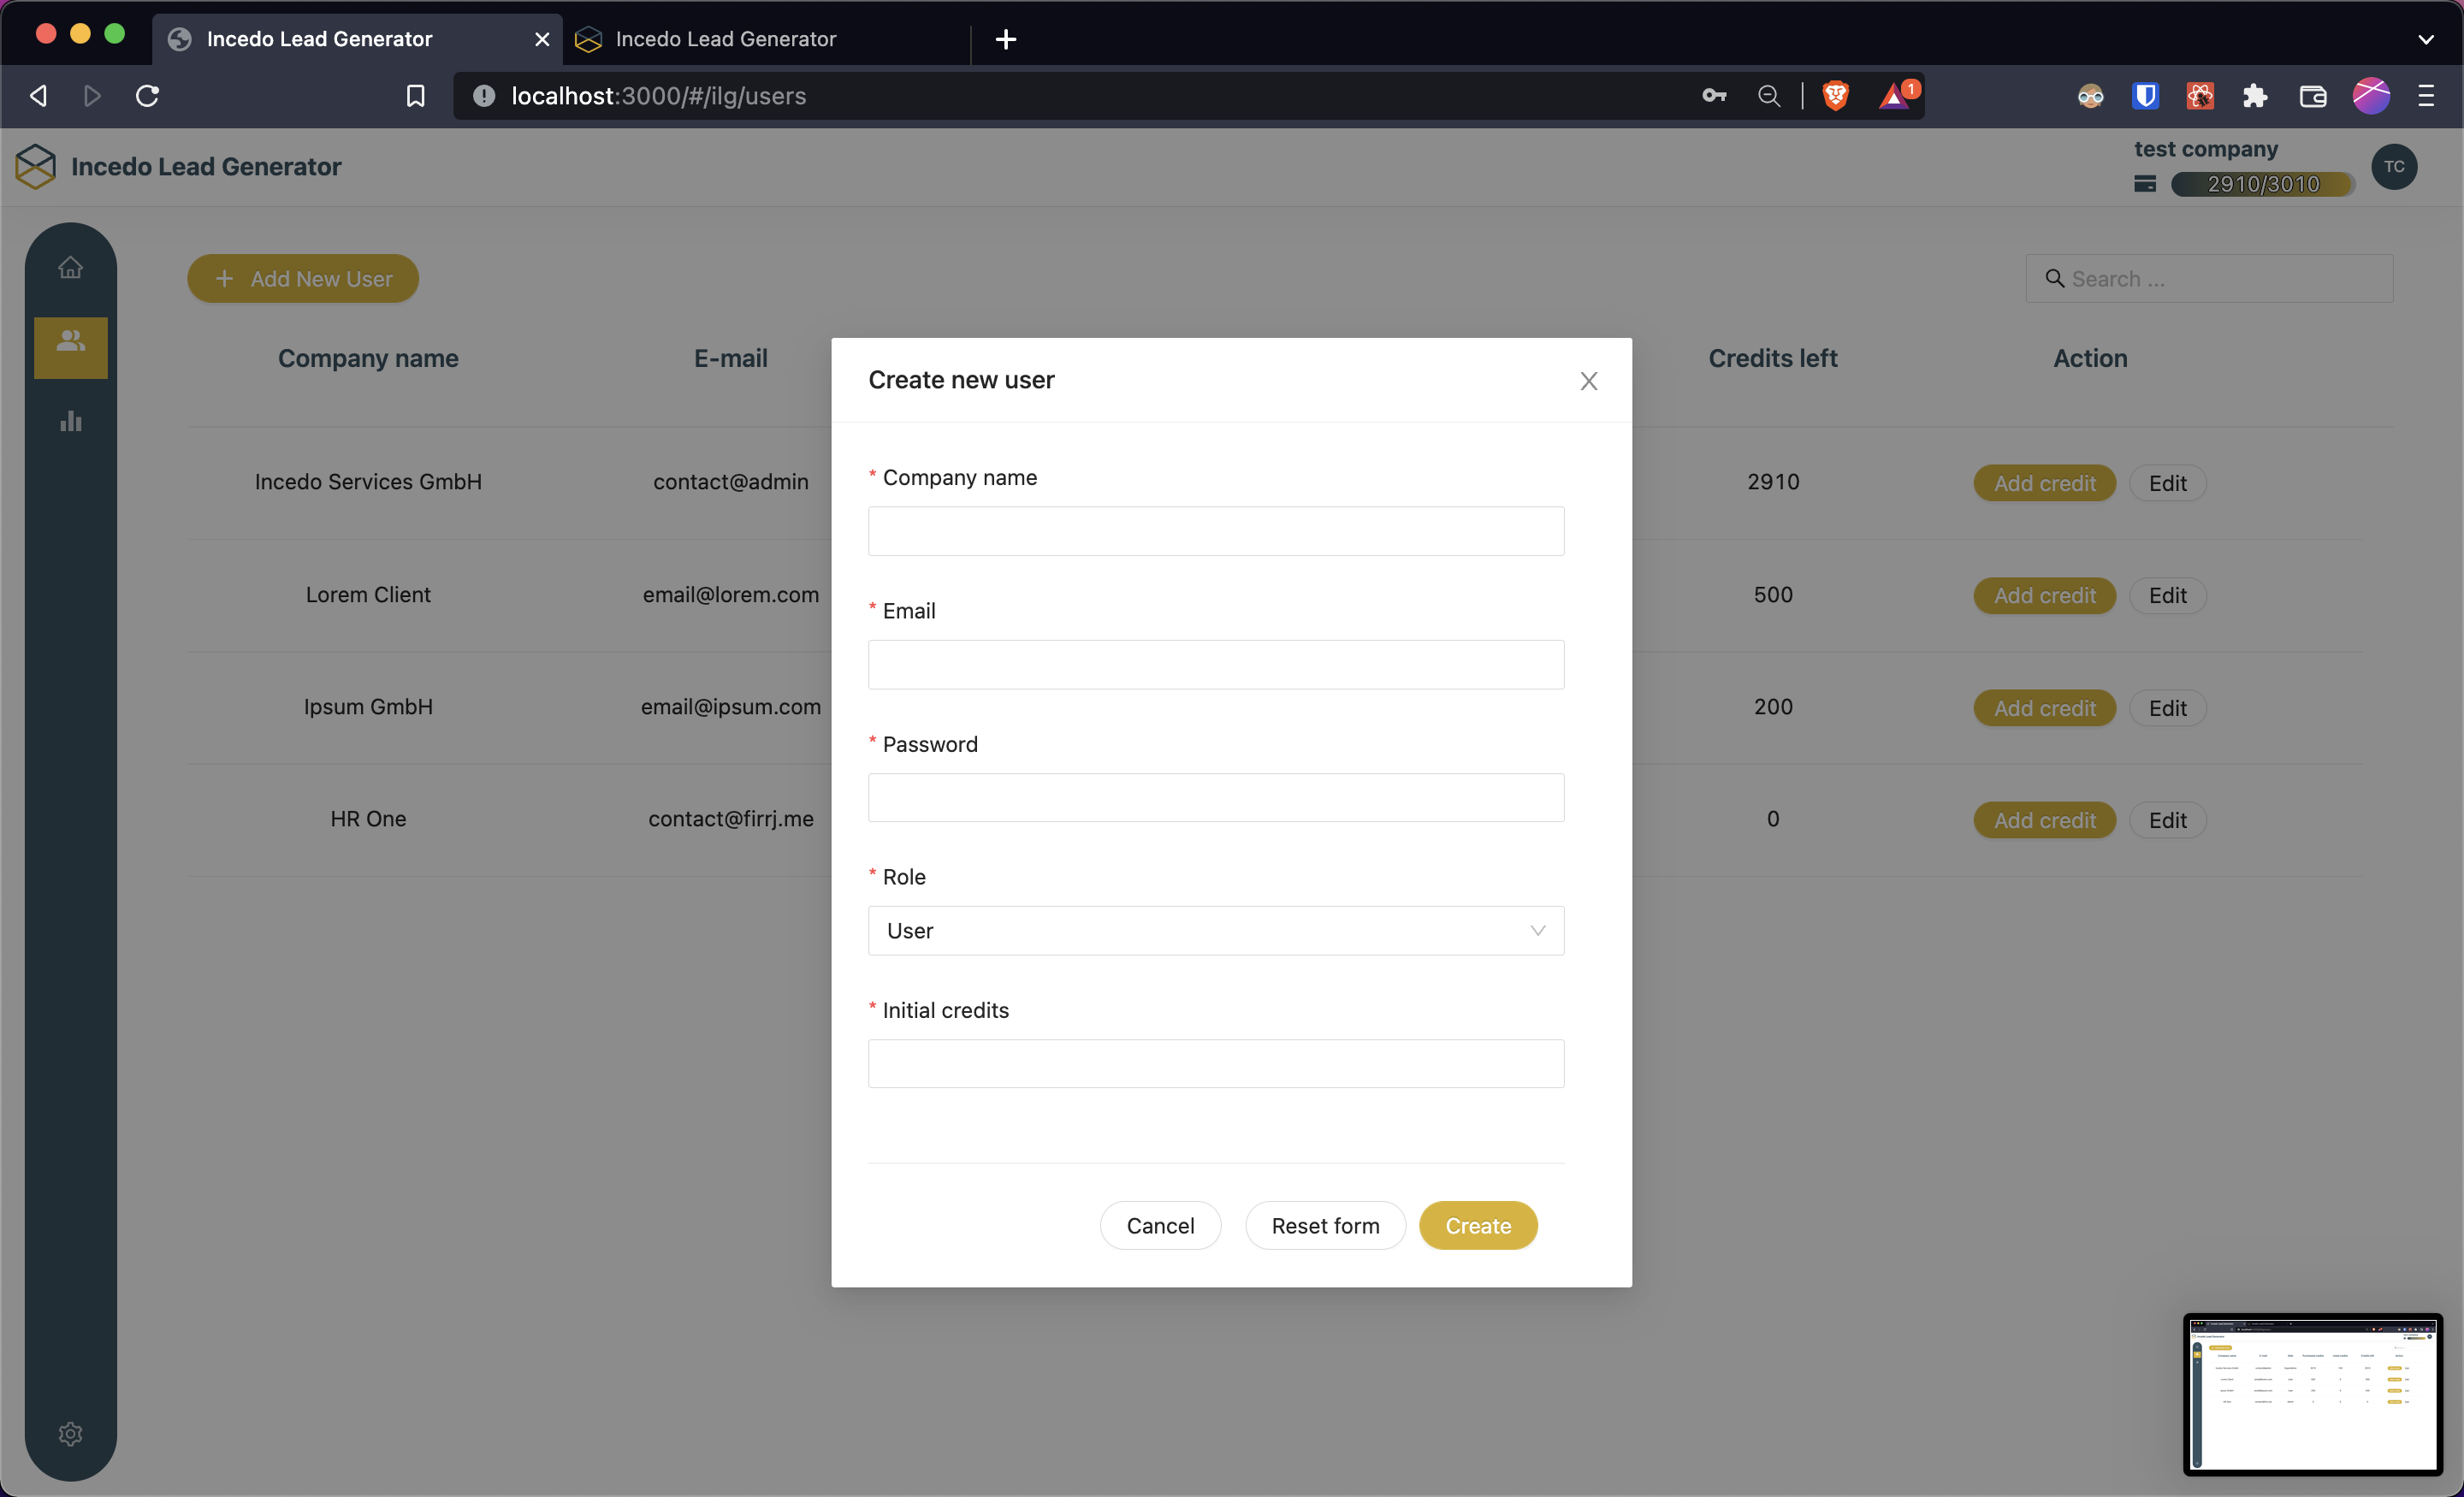
\includegraphics[width=\linewidth]{src/assets/app-screenshots/users-create.png}}
        \caption*{Add User form}
    \end{figure}
    \begin{figure}[H]
        \centering
        \makebox[\textwidth]{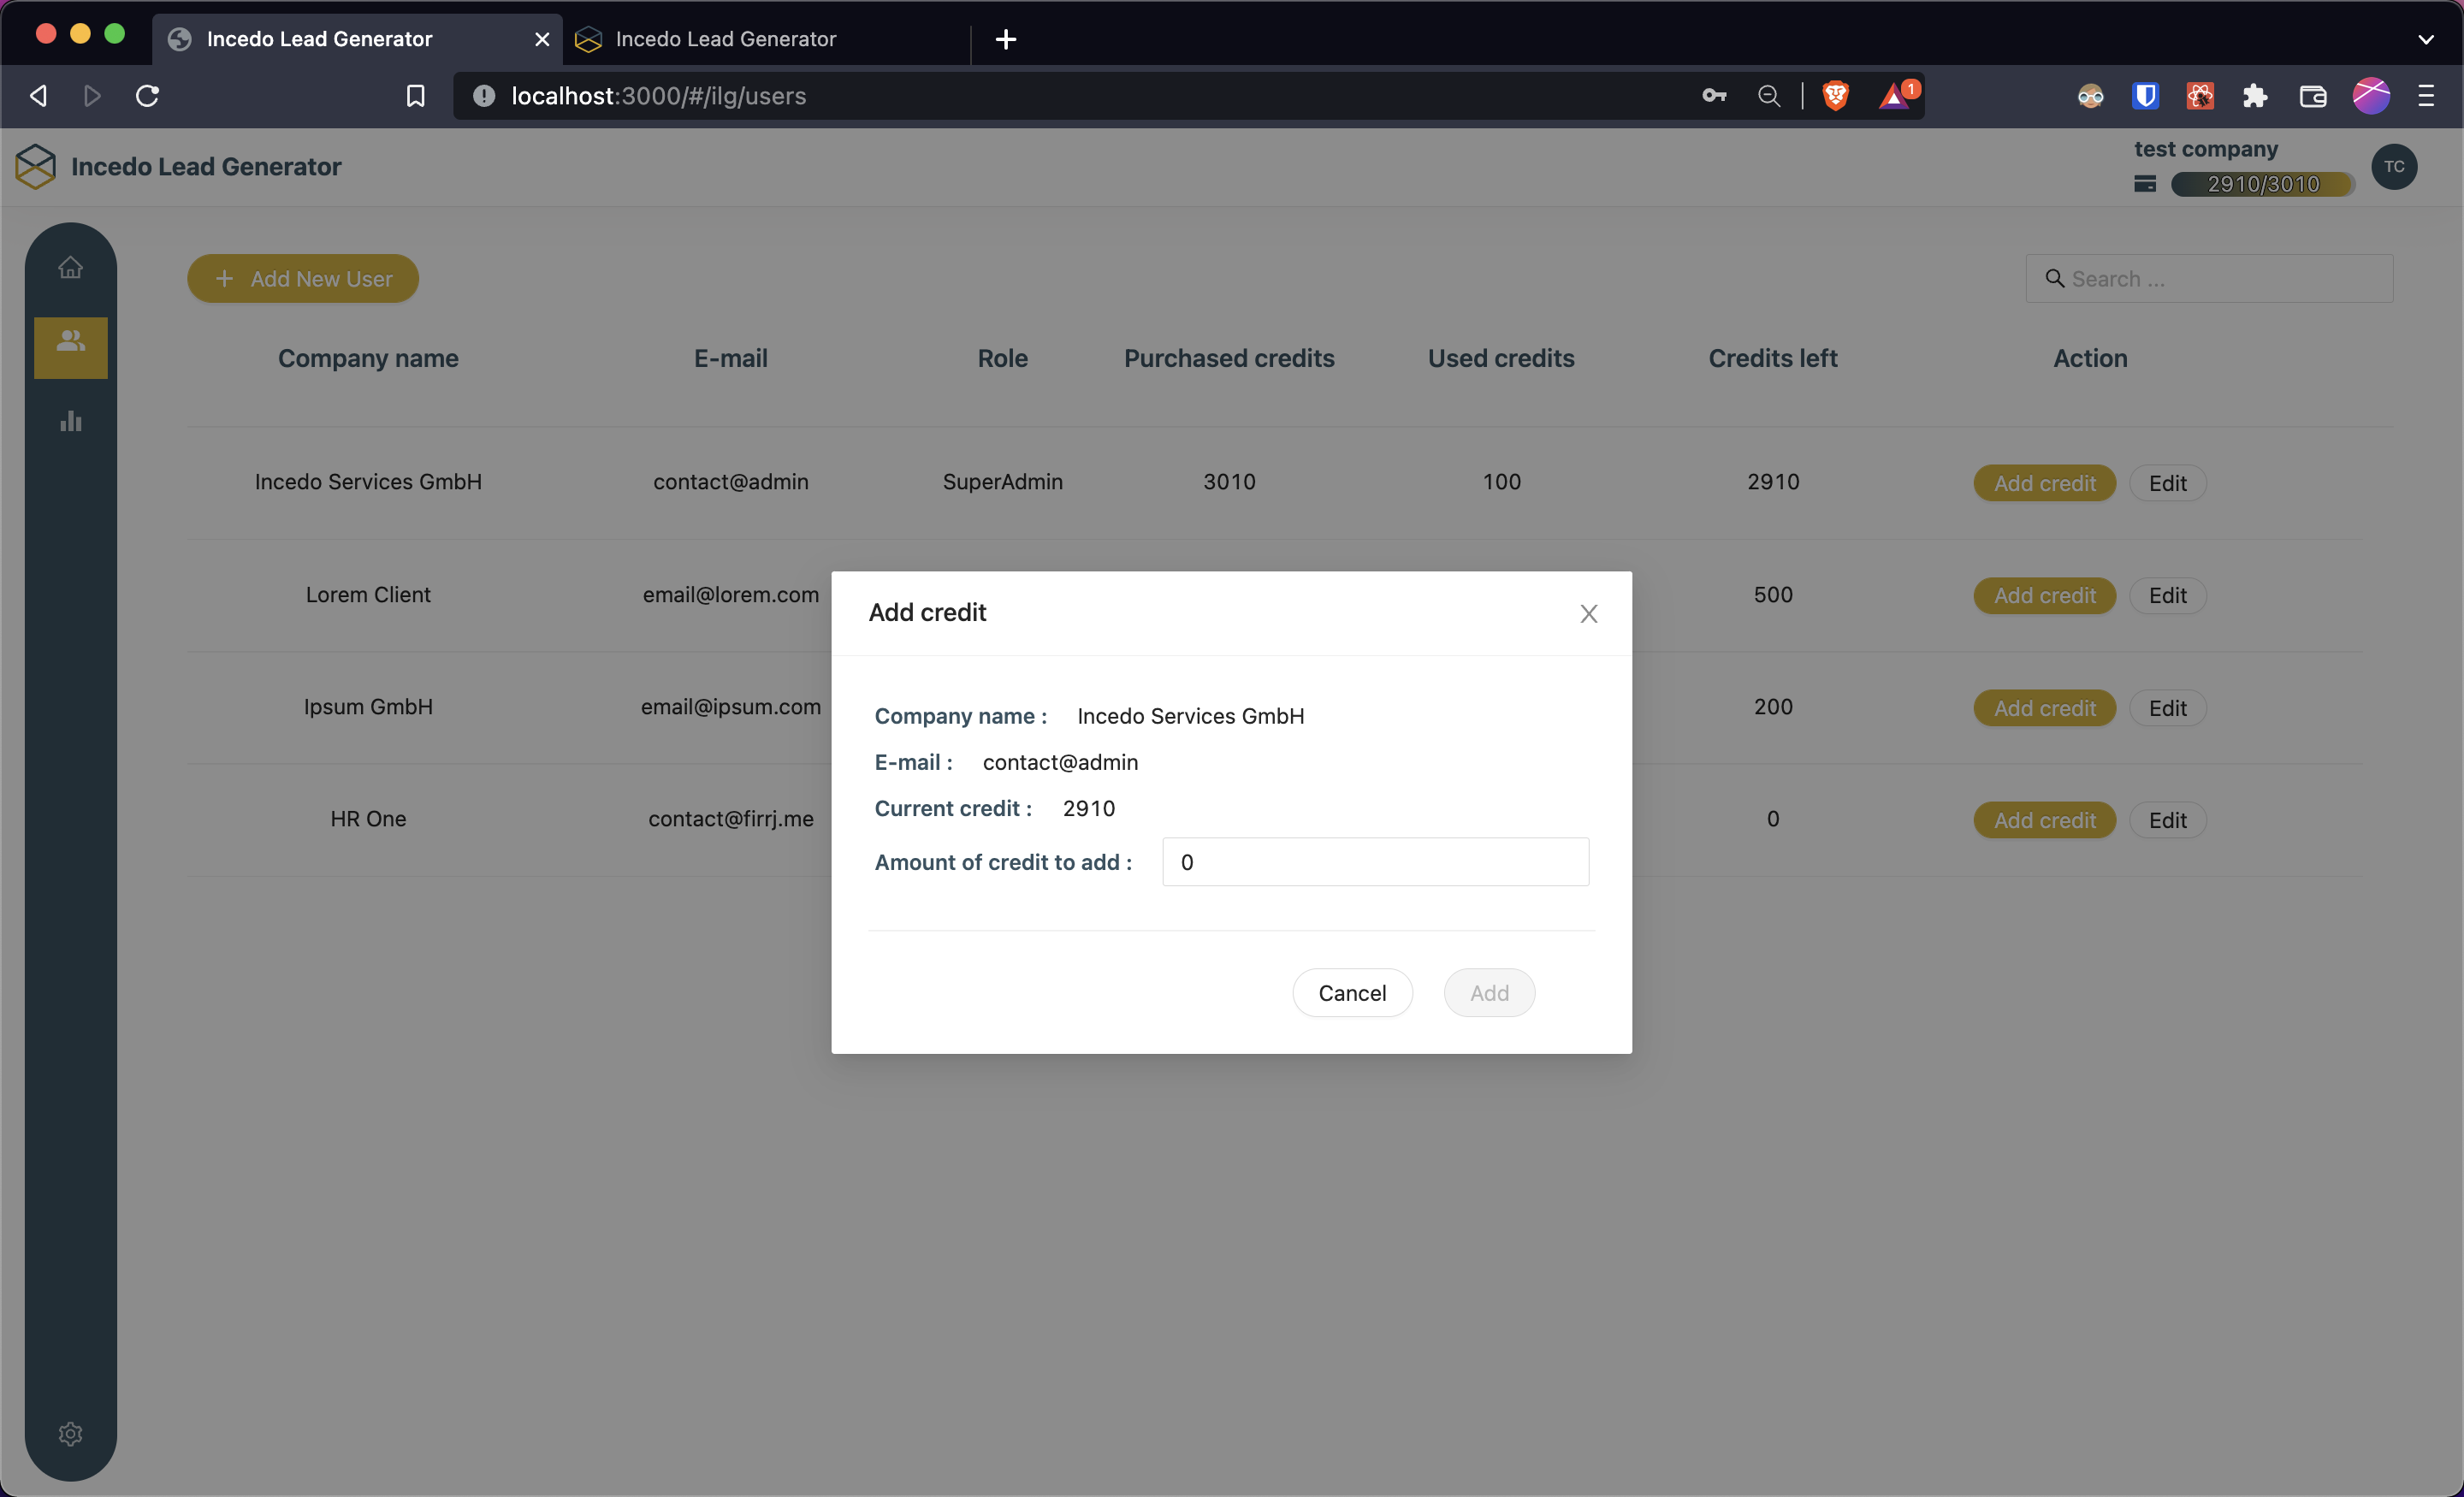
\includegraphics[width=\linewidth]{src/assets/app-screenshots/users-add-credit.png}}
        \caption*{Users Add credit form}
    \end{figure}

    % Appendix c
    \section{Kubernetes dashboard}
    The Kubernetes dashboard is a web based UI for Kubernetes clusters.
    It allows the management of applications running in the cluster.
    \begin{figure}[H]
        \centering
        \makebox[\textwidth]{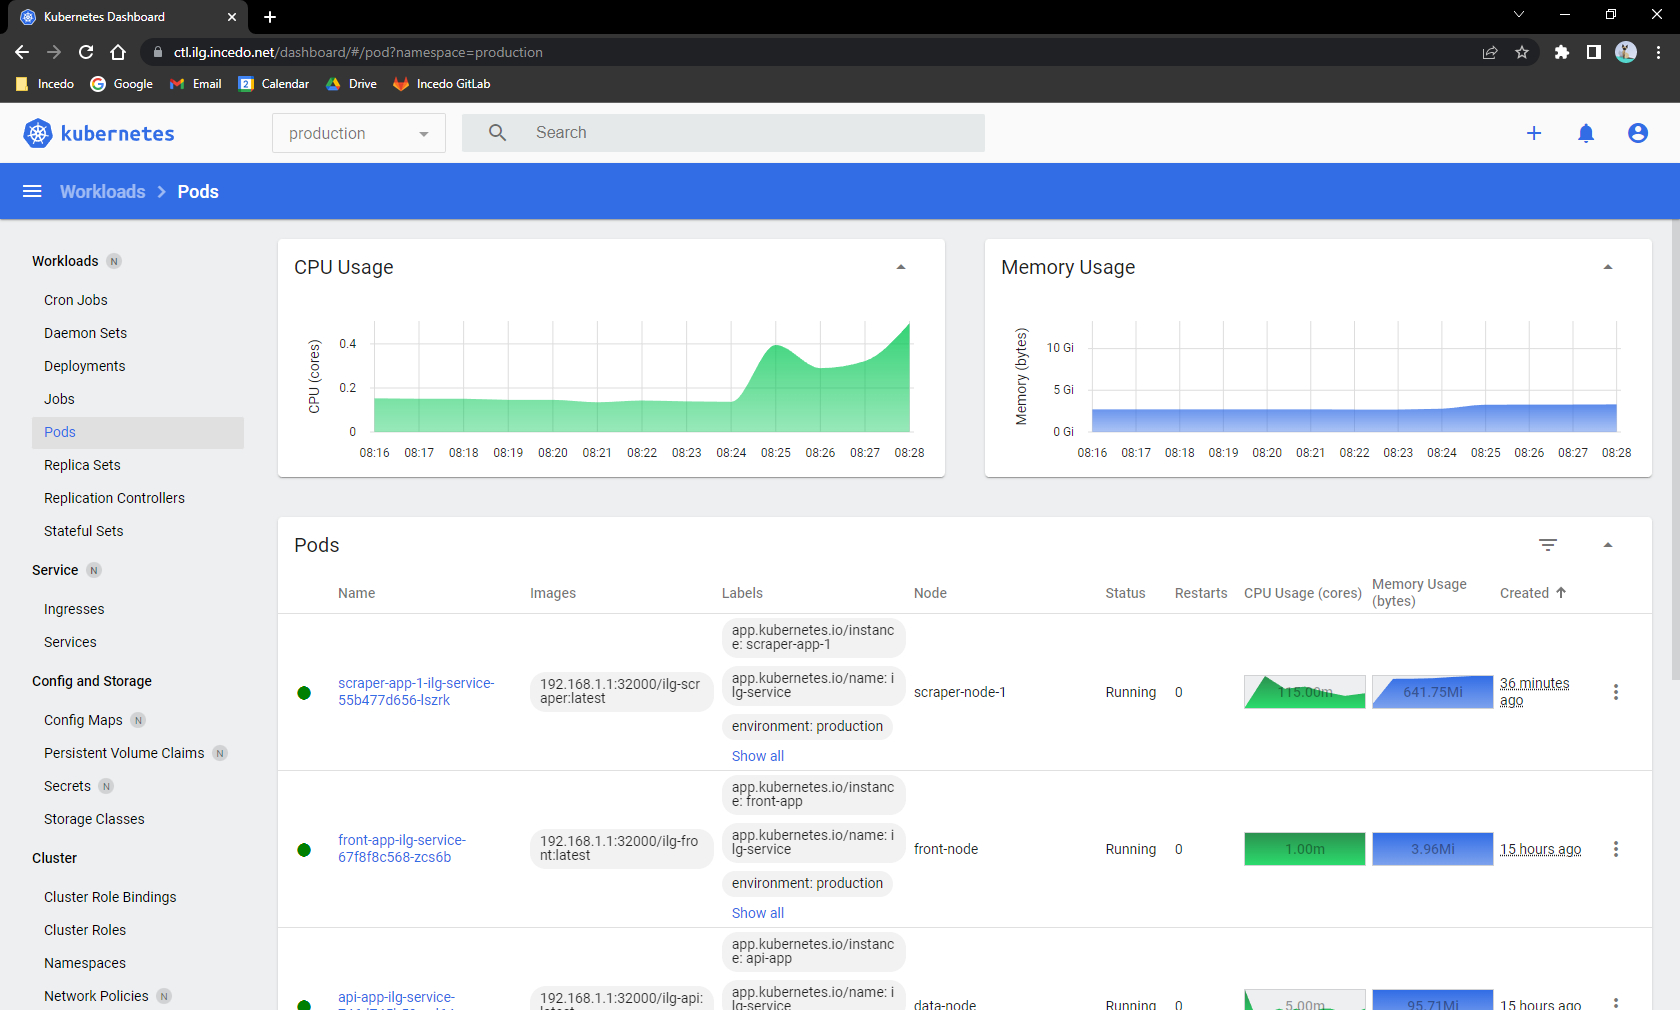
\includegraphics[width=\linewidth]{src/assets/images/kubernetes-dashboard.JPG}}
        \caption*{Monitoring the pods with the Kubernetes dashboard}
    \end{figure}
    \newpage
\end{appendices}


\end{document}
% ------------- Document content ------------- %
